\chapter{Proposta}
\label{chapter:proposta}

Este capítulo descreve e formaliza o sistema proposto por este trabalho. A motivação para este trabalho surgiu a partir de conversas e reuniões com as equipes de desenvolvimento do FloripaSat-2, e tem como inspiração projetos que utilizam conceitos de integração contínua para automatizar o processo de testes e \textit{deploy} de sistemas.

Inicialmente, como teste de conceito, foi criado um \textit{workflow} para automatizar a execução dos testes dos programas de alguns dos subsistemas do satélite, porém, foi feito de um modo genérico o suficiente para que pudesse ser implementado em todos os outro módulos do FloripaSat-2.

Após verificar o funcionamento e a utilidade destes \textit{workflows}, surgiu a possibilidade de aplicar os mesmos conceitos à FlatSat da missão, de modo a automatizar os testes de software e assim, esta se tornou oficialmente a proposta do trabalho.

Os workflows propostos por este trabalho seguirão a mesma linha de raciocínio e apresentarão funcionalidades semelhantes aos já implementados. As próximas seções apresentam uma descrição do modelo proposto, fazendo comparações, quando possível, com o que já foi implementado.


\section{visão geral}
A \textit{FlatSat}, como descrita na seção \ref{section:flatsat}, é uma maneira de testar de maneira rápida e simultânea os subsistemas do satélite. Esta proposta foca em testes de software, utilizando a flatsat como ferramenta de acesso aos sistemas embarcados. Através dela, será possível testar os programas embarcados do FloripaSat-2 de maneira simultânea e em conjunto, analisando a interação entre os diferentes substistemas, além dos funcionamentos isolados.

Estes \textit{workflows} ainda estão em fase de concepção durante a elaboração deste TCC. Por isso, as próximas seções se baseiam nos fluxos de execução já implementados, que possuem muitos dos mesmos objetivos e características de funcionamento.

\section{Workflows}
Esta seção e a próxima tomam como exemplo os workflows de automação empregados no módulo OBDH 2.0, já que os fluxos de automação específicos para a FlatSat serão estruturados de maneira similar e seguindo os mesmos principios. Esta seção apresenta algumas seções de código extraídas para ilustrar e demonstrar o funcionamento do sistema, mas os códigos estão disponíveis de forma pública nos repositórios dos subsistemas, como \cite{eps2-github} e \cite{obdh2-github}. Eles também são apresentados integralmente ao final deste documento, no Apdêndice \ref{cod:obdh_devices}.

    \subsection{Identificação dos Arquivos}
    Os \textit{workflows} são responsáveis por executar uma bateria de testes de unidade, que estão separados em arquivos únicos. Inicialmente, o sistema precisa identificar e compilar cada um desses arquivos de teste. Para isso é empregado um script \textit{Python} que procura nas localizações relevantes arquivos que possuam a nomenclatura apropriada. Neste caso, arquivos cujos nomes terminam como \textit{\_test.c}. O trecho de código abaixo, extraído do arquivo \textit{deployJSON.py} e disponível em \ref{deployJSON.py}, demonstra essa busca pelos arquivos relevantes.

    Os nomes e localização dos testes encontrados são salvos em um arquivo \textit{.json}, utilizado posteriormente para compilação.
    \begin{minted}
        [
        frame=lines,
        framesep=2mm,
        baselinestretch=1.2,
        breaklines=True,
        fontsize=\footnotesize,
        linenos
        ]
        {python}
        for file in file_dir:
        if file.endswith('_test.c'):
            file_name = file.replace('.c', '')
            test_file = file_name.replace('_test', '_unit_test')
            file_path = path + test_file

            file_info = {
                "name": file_name,
                "test_name": test_file,
                "path": file_path
            }

            files['include'].append(file_info)
    \end{minted}

    \subsection{\textit{Job Matrix}}
    Para garantir que os testes sejam executados com relativa rapidez, o \textit{workflow} foi estruturado para executar cada teste simultaneamente de forma isolada. Para isso, foi utilizada uma \textit{Job Matrix}, que se trata de uma maneira de dividir um \textit{workflow} em subtarefas que se excutam paralelamente. Uma explicação detalhada do funcionamento e configuração de uma \textit{Job Matrix} pode ser encontrada na documentação oficial da ferramenta \textit{GitHub Actions} \cite{gh-actions}.

    Neste caso, o número de subtarefas, ou \textit{jobs}, é definido pela quantidade de testes que foram encontrados pelo passo anterior, para que assim o \textit{workflow} gere a matriz através do resultado da execução do script apresentado anteriormente. O Trecho de código a seguir apresenta essa funcionalidade.

    \begin{minted}
        [
        frame=lines,
        framesep=2mm,
        baselinestretch=1.2,
        breaklines=True,
        fontsize=\footnotesize,
        linenos
        ]
        {yaml}

    generate-matrix:
        name:

        runs-on: ubuntu-latest

        outputs:
          matrix: ${{ steps.set-matrix.outputs.matrix }}

        steps:
          # Checks-out the repository under $GITHUB_WORKSPACE, so the job can navigate it
          - uses: actions/checkout@v2

          - name: Create JSON file
            run: python3 .github/workflows/deployJSON.py --source firmware/tests/devices/

          - name: Resulting JSON file for matrix generation
            run: echo "$(cat .github/workflows/test-list.json)"

          # Set the matrix output from the JSON (manipulated to remove spaces and replace \n -> %0A, " -> \")
          - id: set-matrix
            name: Set matrix output from the JSON file
            run: echo "::set-output name=matrix::$( echo "$(cat .github/workflows/test-list.json)" | sed ':a;N;$!ba;s/\n/%0A/g' )"

    \end{minted}


    \subsection{Compilação e execução}
    A compilação é feita através de um comando \textit{make}, recebendo como entrada cada um dos arquivos encontrados pelo script identificador. A Matriz de subtarefas é organizada de modo que os arquivos sejam divididos de maneira única, ou seja, cada subdivisão do \textit{workflow} é responsável por compilar e executar um único teste.
    A figura \ref{fig:workflow_execution_diagram} apresenta um diagrama exemplificando o fluxo de execução do processo descrito. O diagrama não representa a identificação dos arquivos de teste.

    \begin{figure}[!ht]
        \centering
        \caption{Diagrama de execução de um workflow de testes automatizados}
        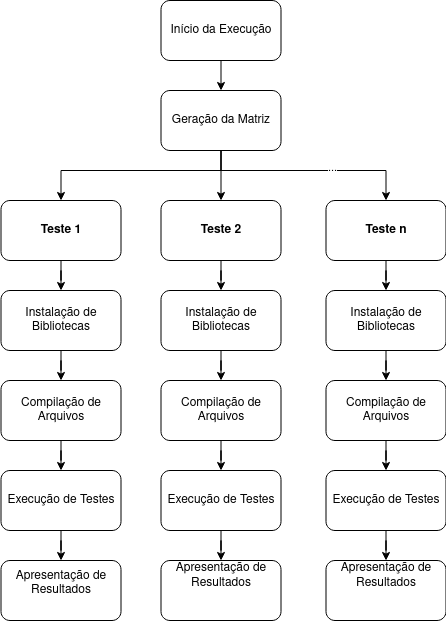
\includegraphics[width=0.8\textwidth]{images/Workflow Execution.drawio.png}
        \legend{Fonte: Autor}
        \label{fig:workflow_execution_diagram}
    \end{figure}

    % \begin{minted}
    % [
    % frame=lines,
    % framesep=2mm,
    % baselinestretch=1.2,
    % breaklines=True,
    % fontsize=\footnotesize,
    % linenos
    % ]
    % {yaml}
    % \end{minted}

\section{\textit{GitHub Actions}}
Esta seção apresenta uma breve descrição da ferramenta \textit{GitHub Actions}, cuja documentação oficial e completa está disponível em \cite{gh-actions}. Ela se uma plataforma de CI/CD (\textit{Continuous Integration/Continuous Delivery}) que permite automatizar testes, builds e deploys através da execução de \textit{workflows} que realizam essas tarefas após alterações no repositório como \textit{commits}, ou \textit{pull requests}.

    \subsection{Hospedagem}
    Os servidores responsáveis pela execução dos \textit{workflows} são chamados de \textit{runners}. O \textit{GitHub} fornece servidores Windows, Ubuntu e macOS, e cada execução de um workflow ocorre em uma máquina virtual nova. Também é possível usar um servidor próprio, chamados de servidores \textit{self-hosted}. Os \textit{workflows} implementados até o momento são executados em servidores Ubuntu do \textit{GitHub}. Os implementados para a FlatSat, no entanto, serão executados em servidores \textit{self-hosted}, já que será necessário manter conexão com os módulos do FloripaSat-2 de modo a testar e executar os programas embarcados.

    \subsection{Execução}
    É possível planejar a execução dos \textit{workflows} e sincronizá-las com ações dentro dos repositórios. Nos casos do OBDH 2.0 e do EPS 2.0, os testes são executados após \textit{commits} em \textit{branches} específicas do repositório como a \textit{master} ou \textit{dev-firmware}, ou após \textit{pull requests}. Também é possível configurar a execução manual, para executar os testes sem realizar nenhuma alteração prévia no repositório.

    \subsection{Resultados}
    Ao fim da execução dos \textit{workflows}, a ferramenta apresenta um \textit{log} com todos os eventos e mensagens retultantes da execução. Aqui é possível, por exemplo, verificar se houve alguma falha na execução dos testes. Esses registros ficam disponíveis no repositório, e sua utilidade vem do nível de detalhamento que forem configurados. Para o sistema proposto por este trabalho, espera-se um elevado nível de detalhamento dos registros, de modo que os resultados possam ser analisados e seja possível extrair dados conclusivos sobre dados de execução e estatística de falhas e sucessos nos testes. A figura \ref{fig:workflow_log} apresenta uma captura de tela de uma execução dos testes durante um \textit{commit} no repositório do OBDH 2.0.

    \begin{figure}[h!]
        \centering
        \caption{Captura de tela do resultado de uma execução de testes automáticos}
        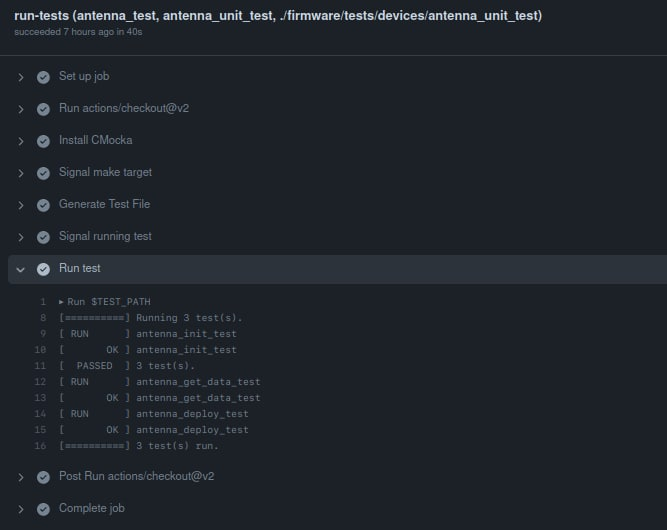
\includegraphics[width=0.9\textwidth]{images/workflow_log.jpg}
        \legend{Fonte: OBDH 2.0 \cite{obdh2-github}}
        \label{fig:workflow_log}
    \end{figure}

\section{Resultados esperados}
Os \textit{workflows} de automação descritos anteriormente se provaram benéficos para o ciclo de desenvolvimento dos sistemas do FloripaSat-2. Através deles, é possível testar cada alteração proposta de maneira eficiente e a automação fornece um registro de execuções passadas, onde é possível comparar alterações no código e os resultados que elas provocaram na execução dos testes. Em termos de controle de versão, os testes foram centralizados e disponibilizados para visualização e estudos.

Espera-se que os programas sob teste na FlatSat possam receber os mesmos benefícios e que isso seja potencializado, visto que o escopo da FlatSat é maior, sendo possível testar não somente a execução individual dos sitemas embarcados, mas também todas as funcionalidades que dependem da integração entre os módulos. Dessa forma, será possível, a princípio, testar o software do FloripaSat-2 como um todo, assumindo que todos os seus substistemas estejam conectados à FlatSat.

Os \textit{workflows} projetados seguirão os mesmos princípios dos que foram descritos anteriormente, de forma a padronizar o uso o dentro da missão e para que seja possível aplicar os mesmos princípios de agilidade e eficiência.

Uma vez que o sistema esteja implementado, espera-se que seu uso contínuo gere uma quantidade considerável de registros e históricos de execução, que serão estudados para produzir a seção de análise deste projeto que trará então um levantamento sobre a utilidade e o impacto do uso desse sistema para o desenvolvimento da missão.
